\documentclass[
	11pt,
]{beamer}

\graphicspath{{Images/}{./}}

\usepackage{booktabs}
\usepackage{bm}
\usepackage{subcaption}
\usepackage{multicol}
\usepackage{amsmath}
\usepackage{biblatex}

\addbibresource{references.bib}

\usetheme{Madrid}

\usefonttheme{default}
\usepackage{palatino}
\usepackage[default]{opensans}

\useinnertheme{circles}

\title[Mathematical Modeling]{Reinforcement Learning with the game Scoundrel}

\author[Colby Cox]{Colby Cox}
\institute[]{University of Central Arkansas}
\date[4/20/2026]{4/20/2026}
\begin{document}

\begin{frame}
	\titlepage
\end{frame}

\begin{frame}
  \frametitle{Objective}
  \begin{itemize}
    \item The original objective was to find an optimized win rate for Scoundrel using reinforcement learning to train an expert agent. This did not work because of the complexity of the observation space and the amount of data needed to play any game of Scoundrel.
    \item The new objective is being able to find a solution to a given deck of cards. This still requires a large amount of data, but is now within a doable range.
  \end{itemize}
\end{frame}

\begin{frame}
  \frametitle{Reinforcement Learning}
  To make decisions, we need to make a policy table $\pi(s, a)$ that maximizes our future reward value $r$. We next define a value function that quantifies the desireability of being in a given state:
  \begin{align*}
    V_\pi(s) = \mathbb{E}\left( \sum_{k=0}^{\infty}\gamma^k r_k | s_0 = s \right)
  \end{align*}
  Eventually, we extract the optimal policy as
  \begin{align*}
    \pi = \arg \max_\pi \mathbb{E} (r_0 + \gamma V(s'))
  \end{align*}
  where $s'$ is our next state.
\end{frame}

\begin{frame}
  \frametitle{Proximal Policy Optimization}
  The goal of PPO is to maximize the following objective function:
  \begin{align*}
    L_t^{CLIP+VF+S}(\theta) = \hat{\mathbb{E}}_t[L_t^{CLIP}(\theta)-c_1L_t^{VF}(\theta)-c_2S[\pi_\theta](s_t)]
  \end{align*}
  where $c_1$ is the VF coeff., $c_2$ is the entropy coeff., $S$ denotes an entropy bonus, and $L_t^{VF}$ is the squared-error loss.
  \begin{align*}
    &L_t^{VF} = (V_\theta(s_t) - V_t^{targ})^2 \\
    &L_t^{CLIP}(\theta) = \hat{\mathbb{E}} \left[ \min(r_t(\theta))\hat{A}_t, \text{clip}(r_t(\theta), 1 - \epsilon, 1 + \epsilon)\hat{A}_t \right]
  \end{align*}
\end{frame}

\begin{frame}
  \small
  \frametitle{Proximal Policy Optimization}
  \hrule
  \vspace{4pt}
  \textbf{Algorithm} PPO, Actor-Critic Style
  \vspace{4pt}
  \hrule
  \vspace{4pt}
  \textbf{for} iteration = 1, 2, ... \textbf{do}

  \hspace{2em} \textbf{for} actor = 1, 2, ... $N$ \textbf{do}

  \hspace{4em} Run policy $\pi_{\theta_\text{old}}$ in environment for $T$ timesteps

  \hspace{4em} Compute advantage estimates for $\hat{A}_1, ..., \hat{A}_T$

  \hspace{2em} \textbf{end for}

  \hspace{2em} Optimize surrogate $L$ wrt $\theta$ with $K$ epochs and minibatch size $M \le NT$

  \hspace{2em} $\theta_\text{old} \leftarrow \theta$

  \textbf{end for}
  \vspace{4pt}
  \hrule
\end{frame}

\begin{frame}
  \frametitle{Action Space}
  The model can choose an integer from 0 to 4 to make its choice.
  \begin{itemize}
    \item If it chooses 0, the player runs.
    \item If it chooses 1-4, then it chooses the card in the position selected.
  \end{itemize}
\end{frame}

\begin{frame}
  \frametitle{Observation Space}
  The observation space is represented by a vector with a length of 8.
  \begin{itemize}
    \item The first 4 values are the current health, the weapon's value, the current monster on the weapon's value, and whether or not the run button is disabled.
    \item The last 4 values represent the state of each of the four cards.
      \begin{itemize}
        \item 0 - There is no card in that slot
        \item 1 - There is a monster in the slot
        \item 2 - There is a weapon in the slot
        \item 3 - There is a health potion in the slot.
      \end{itemize}
  \end{itemize}
\end{frame}

\begin{frame}
  \frametitle{Reward Function}
  There were many attempts to find the reward function
  \begin{enumerate}
    \item Giving a reward of -1000 on a loss and +1000000 on a win.
    \item Giving a reward based on good utilization of the cards. At the end of the turn, it added the health gained and subtracted the damage taken.
    \item Giving a reward based on the distance moved towards the goal from before and after the turn. First, the values of all monsters in the deck and hand are added. Then, the player takes their turn. Finally, previous monster count is subtracted by the current monster count and added as a reward.
  \end{enumerate}
\end{frame}


\begin{frame}
  \frametitle{Results}
  \begin{figure}[h!]
  \centering
  \begin{subfigure}{0.20\textwidth}
    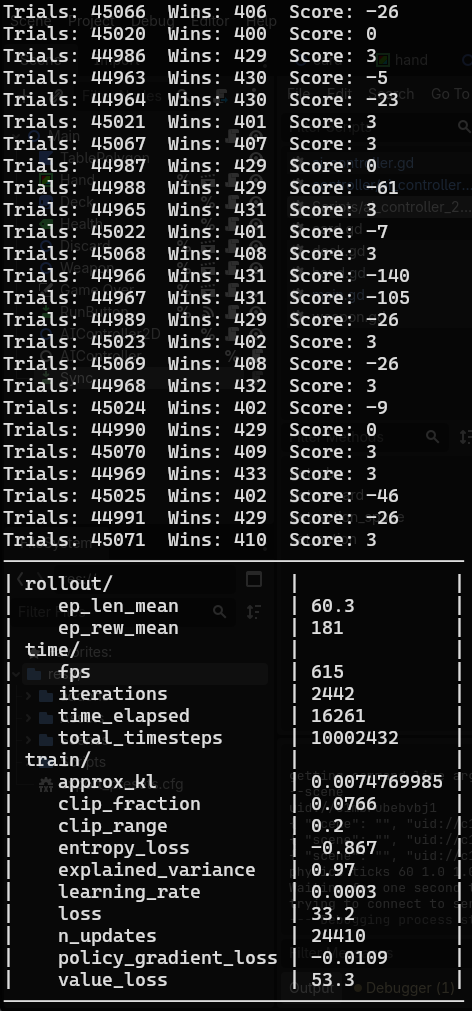
\includegraphics[width=\textwidth]{firstSuccess.png}
    \caption{First Success}
  \end{subfigure}
  \hspace{4pt}
  \begin{subfigure}{0.20\textwidth}
    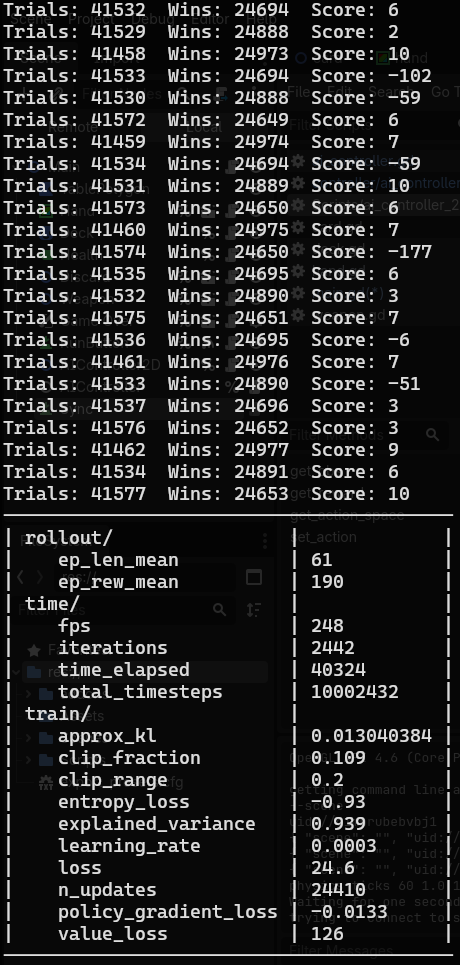
\includegraphics[width=\textwidth]{model.png}
    \caption{First Test}
  \end{subfigure}
  \hspace{4pt}
  \begin{subfigure}{0.2\textwidth}
    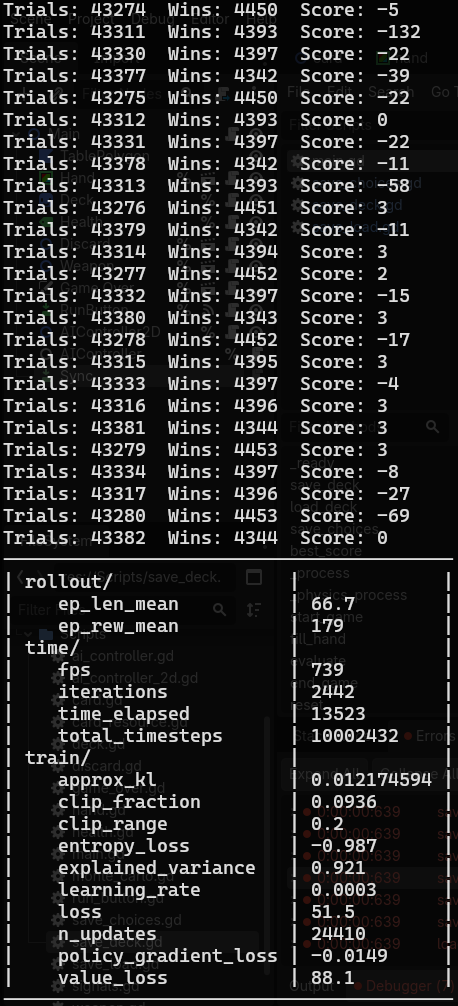
\includegraphics[width=\textwidth]{Trial2.png}
    \caption{Second Test}
  \end{subfigure}
  \hspace{4pt}
  \begin{subfigure}{0.22\textwidth}
    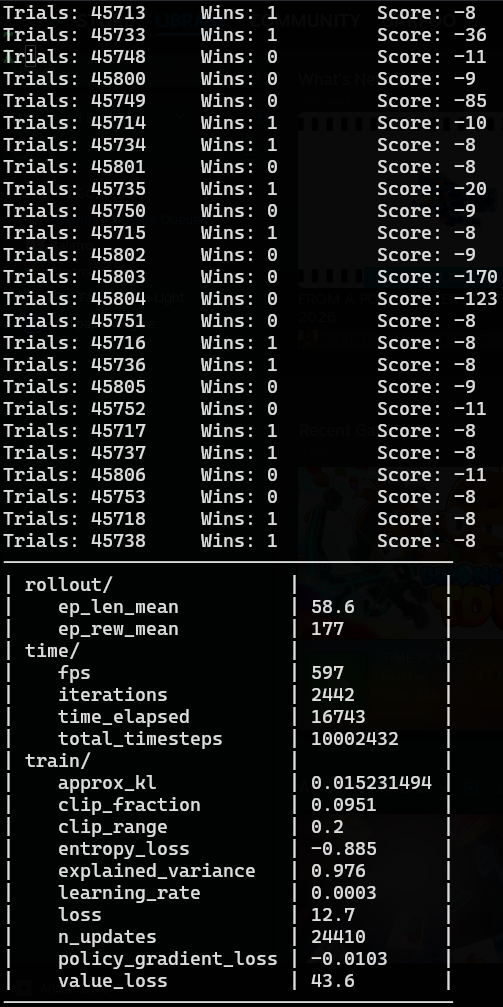
\includegraphics[width=\textwidth]{Trial3.png}
    \caption{Third Test}
  \end{subfigure}
\end{figure}

\end{frame}

\begin{frame}
  \frametitle{Future Considerations}
  There are many ways this project could be improved:
  \begin{itemize}
    \item Hyperparameter tuning
    \item Different algorithms
    \item Optimizing the observation space
    \item Interpreting the decisions of the model
    \item Using exclusively Python
  \end{itemize}
\end{frame}

\begin{frame}[allowframebreaks]
  \frametitle{References}
  \nocite{*}
  \printbibliography
\end{frame}

\end{document}
